\chapter{Contexto}
\label{chap:contexto}

Este capítulo introduz temas que servem como base para a análise e o desenvolvimento presentes nesse estudo.

A seção \ref{sec:ia-na-saude} reflete sobre os avanços, tanto atuais quanto possíveis, providos pela aplicação de inteligência artificial na área de saúde. Em seguida, a seção \ref{sec:algoritmos} explica o funcionamento teórico dos modelos de aprendizado de máquina utilizados no desenvolvimento deste trabalho. Por fim, a seção \ref{sec:trabalhos} contém alguns trabalhos relacionados ao presente estudo, servindo como base acadêmica.


\section{Aprendizado de Máquina na Saúde}
\label{sec:ia-na-saude}

Aprendizado de máquina é um ramo da inteligência artificial e ciência da computação que foca no uso de dados e algoritmos para imitar como os humanos aprendem, melhorando gradativamente sua precisão \cite{ibm}. Algoritmos de aprendizado de máquina são então treinados para reconhecer padrões em dados ou mídias. A partir disso, é possível obter resultados como classificação de dados que não conheciam anteriormente, ou produção de conteúdo se baseando nos padrões percebidos.

Duas áreas da medicina que se beneficiam do aprendizado de máquina são as de diagnóstico e prognóstico de doenças. Diagnóstico consiste em avaliar o estado atual do paciente, tendo visto avanços, por exemplo, utilizar fotos para identificar câncer de pele. Prognóstico consistem em prever a evolução da doença no paciente, como utilizar a coleta de dados de tecnologias vestíveis em pacientes com diabetes para ajudar no tratamento \cite{ml-medicina}.

Uma conquista recente para a medicina veio da rede de inteligência artificial da \textit{Google}, \textit{DeepMind}. Seu algoritmo, \textit{AlphaFold2}, conseguiu prever precisamente a estrutura tridimensional de proteínas a partir da sequência de aminoácidos, um problema enfrentado na área há décadas \cite{deepmind}. Este avanço possibilita um melhor entendimento de como proteínas se comportam e pode trazer uma mudança de paradigma na fabricação de remédios e na compreensão do funcionamento de células \cite{deepmind2}.

O uso de aprendizado de máquina depende da análise de grandes quantidades de dados, mas a emergência de tecnologias vestíveis e sistemas mais distribuídos trazem bons prospectos para seu uso na área de saúde \cite{wearables}.


% \input{chapters/contexto/sections/trabalhos}

\section{Comparação entre Algoritmos}
\label{sec:comparacao-algoritmos}

Após uma certa quantidade de iterações do processo de otimização de parâmetros como especificado na subseção \ref{subsec:otimizacao}, os modelos gerados pelos algoritmos de classificação \textit{k-Nearest Neighbors} (kNN), \textit{Decision Tree} (DT), \textit{Random Forest} (RF), \textit{Gradient Boosting} (GB), \textit{Light Gradient Boosting} (LGB) e \textit{XGBoost} (XGB) %e \textit{Neural Network} (NN)% 
na etapa de treinamento foram aplicados no conjunto de dados de teste.

Cada algoritmo foi executado 20 vezes, aleatorizando o conjunto de dados em cada uma delas, coletando então suas métricas de acurácia, precisão, sensibilidade, \textit{F1-Score} e \textit{AUC-ROC} para cada execução. 
Como discutido na subseção \ref{subsec:calculo-metricas}, as métricas macro representam a média dos resultados de cada classe, que neste conjunto de dados são casos leves e casos graves. 
A média e desvio padrão de cada métrica foi calculada, e as métricas consideradas relevantes para comparação se encontram na tabela \ref{tab:comparacao-algoritmos-normal}, onde o maior valor para cada uma está representado em negrito.

\begin{table}[H]
  \footnotesize
  \centering
  \begin{tabular}{l|c|c|c|c|c|}
  \cline{2-6}
  \textbf{}                          & \textbf{Acurácia}      & \textbf{Precisão Macro} & \textbf{Sensib. Macro} & \textbf{F1-Score Macro} & \textbf{AUC-ROC}       \\ \hline
  \multicolumn{1}{|l|}{\textbf{kNN}} & 0,9790±0,0001          & 0,9475±0,0007           & 0,8228±0,0020          & 0,8739±0,0011           & 0,8228±0,0020          \\ \hline
  \multicolumn{1}{|l|}{\textbf{DT}}  & 0,9767±0,0015          & 0,9558±0,0133           & 0,7913±0,0094          & 0,8534±0,0101           & 0,7913±0,0094          \\ \hline
  \multicolumn{1}{|l|}{\textbf{RF}}  & 0,9828±0,0001          & \textbf{0,9795±0,0006}  & 0,8395±0,0012          & 0,8962±0,0009           & 0,8395±0,0012          \\ \hline
  \multicolumn{1}{|l|}{\textbf{GB}}  & 0,9835±0,0002          & 0,9727±0,0022           & 0,8513±0,0015          & 0,9020±0,0012           & 0,8513±0,0015          \\ \hline
  \multicolumn{1}{|l|}{\textbf{LGB}} & 0,9835±0,0002          & 0,9748±0,0016           & 0,8498±0,0015          & 0,9018±0,0001           & 0,8498±0,0015          \\ \hline
  \multicolumn{1}{|l|}{\textbf{XGB}} & \textbf{0,9838±0,0003} & 0,9707±0,0010           & \textbf{0,8571±0,0031} & \textbf{0,9052±0,0022}  & \textbf{0,8571±0,0031} \\ \hline 
\end{tabular}
\caption{Médias de métricas de algoritmos de classificação na etapa de teste}
\label{tab:comparacao-algoritmos-normal}
\end{table}

Levando em consideração a métrica \textit{AUC-ROC} como métrica de avaliação, é possível observar que, enquanto todos os algoritmos alcançaram um valor próximo ou acima de 80\%, o algoritmo \textit{XGBoost} obteve o melhor desempenho, bem próximo dos outros algoritmos de \textit{Gradient Boosting}. O \textit{F1-Score Macro} também é um indicador de desempenho satisfatório, e todos os algoritmos alcançaram valores acima de 85\%, com os algoritmos baseados em \textit{Gradient Boosting} alcançando valores acima de 90\%. 

Embora a Precisão Macro tenha alcançado valores altos, até acima de 97\%, a Sensibilidade Macro ficou sempre abaixo dos 90\%, devido a uma quantidade considerável de falsos negativos, casos graves classificados como leves. É possível observar este resultado na tabela \ref{tab:matriz-confusao-xgboost}, que mostra a matriz de confusão do \textit{XGBoost} com melhor \textit{F1-Score} das 20 execuções, 90,97\%.

\begin{table}[H]
  \footnotesize
  \centering
  \centering
  \begin{tabular}{l|c|c|}
    \cline{2-3}
    \textbf{}                         & \multicolumn{1}{l|}{\textbf{Predição: LEVE}} & \multicolumn{1}{l|}{\textbf{Predição: GRAVE}} \\ \hline
    \multicolumn{1}{|l|}{\textbf{Real: LEVE}}  & 114511                                       & 205 (0,18\%)                                           \\ \hline
    \multicolumn{1}{|l|}{\textbf{Real: GRAVE}} & 1664 (27,07\%)                                         & 4483                                          \\ \hline   
  \end{tabular}
  \caption{Matriz de confusão de uma execução do \textit{XGBoost}}
  \label{tab:matriz-confusao-xgboost}
\end{table}

Tomando a tabela \ref{tab:matriz-confusao-xgboost} como exemplo, somente 0,18\% de casos leves foram preditos como graves, um número ínfimo de falsos negativos. Isso significa que existe uma confiabilidade satisfatória nos casos preditos como graves. 

Contudo, 27\% dos casos graves foram erroneamente preditos como leves, significando que cerca de 1/4 dos casos graves não foram percebidos pelo algoritmo. Este fenômeno se mostrou presente em todos os algoritmos analisados, sendo a causa da diminuição da Sensibilidade Macro observada na tabela \ref{tab:comparacao-algoritmos-normal}.

Este problema ocorre devido ao desbalanceamento do conjunto de dados, onde existem 20x mais casos leves que graves. Portanto, durante a etapa de otimização de parâmetros descrita na subseção \ref{subsec:otimizacao}, técnicas de balanceamento de dados foram utilizadas. O processo de balanceamento consiste em igualar a quantidade de classes no conjunto de dados, excluindo registros aleatórios da classe mais comum. Os resultados se encontram na tabela \ref{tab:comparacao-algoritmos-undersample}.

\begin{table}[H]
  \footnotesize
  \centering
  \begin{tabular}{l|c|c|c|c|c|}
  \cline{2-6}
  \textbf{}                          & \textbf{Acurácia}      & \textbf{Precisão Macro} & \textbf{Sensib. Macro} & \textbf{F1-Score Macro} & \textbf{AUC-ROC}       \\ \hline
  \multicolumn{1}{|l|}{\textbf{kNN}} & 0,9047±0,0027          & 0,9050±0,0026           & 0,9047±0,0027          & 0,9047±0,0027           & 0,9047±0,0027          \\ \hline
  \multicolumn{1}{|l|}{\textbf{DT}}  & 0,8896±0,0102          & 0,8905±0,0096           & 0,8896±0,0102          & 0,8895±0,0103           & 0,8896±0,0102          \\ \hline
  \multicolumn{1}{|l|}{\textbf{RF}}  & 0,9150±0,0019          & 0,9158±0,0020           & 0,9150±0,0019          & 0,9150±0,0019           & 0,9150±0,0019          \\ \hline
  \multicolumn{1}{|l|}{\textbf{GB}}  & 0,9234±0,0022          & 0,9238±0,0022           & 0,9234±0,0022          & 0,9234±0,0022           & 0,9234±0,0022          \\ \hline
  \multicolumn{1}{|l|}{\textbf{LGB}} & 0,9233±0,0009          & 0,9239±0,0009           & 0,9233±0,0009          & 0,9233±0,0009           & 0,9233±0,0009          \\ \hline
  \multicolumn{1}{|l|}{\textbf{XGB}} & \textbf{0,9243±0,0016} & \textbf{0,9249±0,0013}  & \textbf{0,9243±0,0016} & \textbf{0,9242±0,0016}  & \textbf{0,9243±0,0016} \\ \hline
\end{tabular}
\caption{Médias de métricas de algoritmos de classificação na etapa de testes com classes balanceadas}
\label{tab:comparacao-algoritmos-undersample}
\end{table}

A Sensibilidade Macro teve um aumento considerável, chegando acima dos 90\% na maioria dos algoritmos, enquanto a Precisão Macro sofreu uma queda. O \textit{F1-Score} consequentemente teve um aumento, por ser a média harmônica dessas medidas. A acurácia caiu significativamente, não mais inflada pelos casos leves, enquanto o valor \textit{AUC-ROC} cresceu proporcionalmente. Demonstram-se essas diferenças mais detalhadamente na tabela \ref{tab:matriz-confusao-xgboost-undersample}, uma matriz de confusão do XGBoost com \textit{F1-Score} de 92,67\%.

\begin{table}[H]
  \footnotesize
  \centering
  \centering
  \begin{tabular}{l|c|c|}
    \cline{2-3}
    \textbf{}                         & \multicolumn{1}{l|}{\textbf{Predição: LEVE}} & \multicolumn{1}{l|}{\textbf{Predição: GRAVE}} \\ \hline
    \multicolumn{1}{|l|}{\textbf{Real: LEVE}}  & 5770                                       & 377 (6,13\%)                                           \\ \hline
    \multicolumn{1}{|l|}{\textbf{Real: GRAVE}} & 524 (8,52\%)                                         & 5623                                          \\ \hline   
  \end{tabular}
  \caption{Matriz de confusão de uma execução do \textit{XGBoost} com classes balanceadas}
  \label{tab:matriz-confusao-xgboost-undersample}
\end{table}

Neste cenário, a diferença entre a proporção de falsos positivos e falsos negativos se equilibra, ainda que se mantenha maior nos casos graves. Existe uma chance de que casos leves sejam preditos como graves, mas a chance de que casos graves sejam preditos como leves é muito menor que anteriormente. Considerando a natureza médica do problema, uma menor taxa de casos graves perdidos pode ser considerada uma melhoria significativa, mesmo que exista um aumento na quantidade de alarmes falsos para casos leves \cite{medical-ai-measure}. Portanto, assimilando este julgamento ao aumento do valor \textit{AUC-ROC}, escolhido como métrica de desempenho, balancear o conjunto de dados por \textit{RandomUnderSampler} se evidencia como uma melhoria.


\section{Métricas de Desempenho}
\label{sec:metricas}

Para comparar os resultados obtidos com os algoritmos de classificação, são utilizadas métricas de desempenho. As predições dos algoritmos são comparadas com os valores reais do conjunto de dados, e a métrica de desempenho é calculada com base nesses valores. As subseções a seguir explicam cada métrica com um exemplo.

\subsection{Matriz de Confusão}
\label{subsec:matriz-confusao}

A matriz de confusão é uma tabela que mostra a quantidade de acertos e erros de cada algoritmo para cada classe \cite{confusion}.

\begin{table}[H] 
  \centering
  \begin{tabular}{l|c|c|}
    \cline{2-3}
    \textbf{}                         & \multicolumn{1}{l|}{\textbf{Predição: LEVE}} & \multicolumn{1}{l|}{\textbf{Predição: GRAVE}} \\ \hline
    \multicolumn{1}{|l|}{\textbf{Real: LEVE}}  & 114631                                       & 85                                            \\ \hline
    \multicolumn{1}{|l|}{\textbf{Real: GRAVE}} & 1949                                         & 4198                                          \\ \hline
  \end{tabular}
  \caption{Exemplo de matriz de confusão binária}
  \label{tbl:tabela-matriz-confusao-metricas} 
\end{table}

O valor na primeira célula, \textbf{Predição: LEVE} e \textbf{Real: LEVE}, indica a quantidade de acertos para a classe LEVE, ou Verdadeiro Positivo (TP), com 114631 acertos. Assim, o valor da segunda célula, \textbf{Predição: GRAVE} e \textbf{Real: LEVE}, indica quantos casos leves foram preditos como graves, chamados de Falsos Positivos (FP), totalizando 85 erros nesta classe.

Da mesma forma, o valor de \textbf{Predição: GRAVE} e \textbf{Real: GRAVE}, indica que houveram 4198 acertos na classe de casos graves, chamados de Verdadeiros Negativos (TN). Igualmente, \textbf{Predição: LEVE} e \textbf{Real: GRAVE} indica quantos casos graves foram preditos como leves, chamados de Falsos Negativos (FN), com 1949 casos graves preditos como leves, uma quantidade considerável e de grande relevância para o problema em questão.

Destes valores, é possível, por meio de cálculos, obter as seguintes métricas.

\begin{table}[H]
  \centering
  \begin{tabular}{c|c|c|c}
    \cline{2-3}
    \textbf{} & \textbf{Positivo Predito} & \textbf{Negativo Predito}         & \textbf{}                              \\ \hline
    \multicolumn{1}{|c|}{\textbf{\begin{tabular}[c]{@{}c@{}}Positivo\\ Predito\end{tabular}}} &
      \begin{tabular}[c]{@{}c@{}}TP\\ 114631\end{tabular} &
      \begin{tabular}[c]{@{}c@{}}FN\\ 85\end{tabular} &
      \multicolumn{1}{c|}{\textit{Sensibilidade}} \\ \hline
    \multicolumn{1}{|c|}{\textbf{\begin{tabular}[c]{@{}c@{}}Negativo\\ Predito\end{tabular}}} &
      \begin{tabular}[c]{@{}c@{}}FP\\ 1949\end{tabular} &
      \begin{tabular}[c]{@{}c@{}}TN\\ 4198\end{tabular} &
      \multicolumn{1}{c|}{\textit{Especificidade}} \\ \hline
    \textbf{} & \textit{Precisão}         & \textit{Valor Preditivo Negativo} & \multicolumn{1}{c|}{\textit{Acurácia}} \\ \cline{2-4} 
  \end{tabular}
  \caption{Exemplo de métricas de uma matriz de confusão binária}
  \label{tbl:tabela-matriz-confusao-metricas-explicado}  
\end{table}

\subsection{Acurácia}
\label{subsec:acuracia}

A acurácia indica a quantidade de casos que foram preditos corretamente.

  \begin{equation}
    \textbf{Acurácia} = \frac{TP + TN}{TP + TN + FP + FN}
  \end{equation}

Portanto, a execução do \textit{Random Forest} de exemplo, com a matriz de confusão acima, obteve uma acurácia de 0,98317, ou 98,317\%.

\subsection{Precisão}
\label{subsec:precisao}

A precisão indica a quantidade de casos leves que foram preditos corretamente, dividido pelo total de predições positivas. Essa métrica serve para o julgamento da veracidade dos casos leves preditos, porém ignora os casos graves.

  \begin{equation}
    \textbf{Precisão} = \frac{TP}{TP + FP}
  \end{equation}

Assim, a execução de exemplo obteve uma precisão de 98,328\%.

\subsection{Valor Preditivo Negativo}
\label{subsec:valor-preditivo-negativo}

A precisão também pode ser chamada de valor preditivo positivo, então o valor preditivo negativo é a precisão dos casos negativos, ou casos graves, indicando a quantidade de casos graves que foram preditos corretamente, divido pelo total de predições negativas. Da mesma forma, a métrica ignora os casos leves, mas traz confiança que os casos graves são realmente graves.

  \begin{equation}
    \textbf{Valor Preditivo Negativo} = \frac{TN}{TN + FN}
  \end{equation}

A execução de exemplo obteve um valor preditivo negativo de 98,015\%

\subsection{Precisão Macro}
\label{subsec:precisao-macro}

É possível utilizar a precisão de cada classe para calcular a precisão macro. Em conjuntos com apenas duas classes, a precisão macro é a média da precisão e do valor preditivo negativo, sendo mais dinâmica.

  \begin{equation}
    \textbf{Precisão Macro} = \frac{1}{N}\sum_{i=1}^{N}\frac{TP_{i}}{TP_{i} + FP_{i}}
  \end{equation}

A média das métricas então resulta em 98,171\%.


\subsection{Sensibilidade}
\label{subsec:sensibilidade}

\textit{Recall}, ou sensibilidade, indica a quantidade de casos leves que foram preditos corretamente, dividido pelo total de casos leves. A sensibilidade então serve como uma medida de que as predições não vão resultar em alarmes falsos, prevendo casos leves como graves.

  \begin{equation}
    \textbf{Sensibilidade} = \frac{TP}{TP + FN}
  \end{equation}

Obtendo um valor de 99,925\%, com uma baixa quantidade de falsos negativos.

\subsection{Especificidade}
\label{subsec:especificidade}

A especificidade indica a quantidade de casos graves que foram preditos corretamente, dividido pelo total de casos graves. É equivalente à sensibilidade dos casos graves, medindo os casos graves que foram julgados como LEVE, com grande relevância para o conjunto de dados em questão.

  \begin{equation}
    \textbf{Especificidade} = \frac{TN}{TN + FP}
  \end{equation}

Obtendo um valor de 68,293\%, relativamente baixa confiança em casos graves, significando que mais de 30\% dos casos graves não foram classificados corretamente.

\subsection{Sensibilidade Macro}
\label{subsec:sensibilidade-macro}

Similar à precisão macro, a sensibilidade macro é a média da sensibilidade e da especificidade em conjuntos de dados binários, medindo os falsos positivos e falsos negativos.

  \begin{equation}
    \textbf{Sensibilidade Macro} = \frac{1}{N}\sum_{i=1}^{N}\frac{TP_{i}}{TP_{i} + FN_{i}}
  \end{equation}

A média então resulta em 84,109\%, que, em comparação com a sensibilidade, informa que a especificidade está baixa.

\subsection{F1-Score}
\label{subsec:f1-score}

O \textit{F1-Score}, ou F1, é uma métrica composta que utiliza a média harmônica da precisão e da sensibilidade, de forma a medir tanto predições corretas quanto predições falsas dos casos leves.

\begin{equation}
  \textbf{F1-Score} = 2\times\frac{Precis.\times Sensib.}{Precis. + Sensib}
\end{equation}

Alternativamente:
\begin{equation}
  \textbf{F1-Score} = \frac{2TP}{2TP + FP + FN}
\end{equation}

Assim obtendo um valor de 99,120\%, um valor alto, demonstrando que as predições de casos leves são confiáveis.
A mesma métrica pode ser aplicada à classe de casos graves, resultando em 80,5\%, um valor bem mais baixo em comparação.

\subsection{F1-Score Macro}
\label{subsec:f1-score-macro}

É possível então utilizar o \textit{F1-score} de cada classe para calcular o \textit{F1-score} macro, levando em conta não só a precisão e a sensibilidade, mas também o valor preditivo negativo e a especificidade, sendo uma média entre os \textit{F1-scores} das classes.

  \begin{equation}
    \textbf{F1-Score Macro} = \frac{1}{N}\sum_{i=1}^{N}\frac{2TP_{i}}{2TP_{i} + FP_{i} + FN_{i}}
  \end{equation}

Obtendo-se assim um valor que considera todas as métricas anteriores, 89,810\%, trazendo uma visão mais ampla do desempenho do algoritmo em questão.

\subsection{AUC ROC}
\label{subsec:curva-roc}

Além do \textit{F1-score}, é possível utilizar as métricas calculadas para plotar a curva Característica de Operação do Receptor (ROC), tendo a sensibilidade no eixo Y contra a especificidade invertida no eixo X. A curva permite não só visualizar o desempenho do classificador e encontrar o ponto ótimo da sensibilidade em função da especificidade, sendo o ponto mais próximo da esquerda superior \cite{roc}.

\begin{figure}[ht!]
  \centering
  \fcolorbox{white}{white}{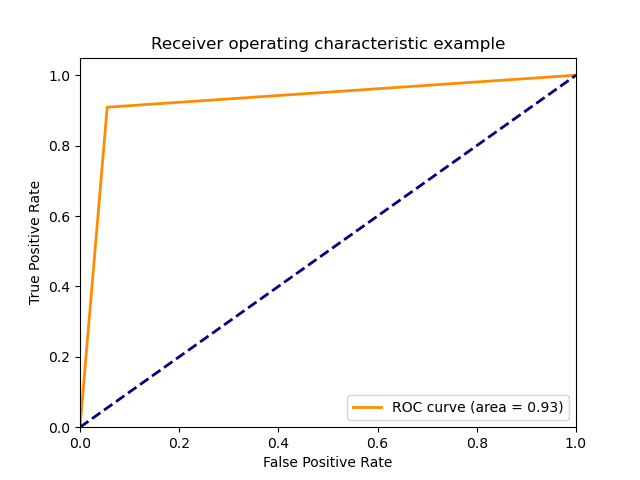
\includegraphics[width=0.5\textwidth]{chapters/metodologia/images/roc.png}}
  \caption{\textmd{Curva ROC de uma execução de XGBoost}}
  \label{fig:curva-roc-exemplo}
\end{figure}

Com a curva, é possível então calcular a Área Abaixo da Curva (AUC), onde um modelo com 0\% de acurácia teria um AUC de 0, e um modelo com 100\% de acurácia teria um AUC de 1. Na figura \ref{fig:curva-roc-exemplo}, o modelo de exemplo alcançou um AUC de 93,768\%.


\section{Trabalhos Relacionados}
\label{sec:trabalhos}

Considerando a relevância de aplicar inteligência artificial na área de saúde e a urgência em escala global da pandemia de COVID-19, uma miríade de estudos sobre o tema foram publicados, tanto internacionalmente quanto no Brasil. Alguns trabalhos relacionados ao presente estudo são descritos a seguir. O valor \textit{AUC-ROC}, discutido na subseção \ref{subsec:calculo-metricas}, será utilizado como principal métrica de desempenho entre trabalhos.

\subsection{Trabalhos Internacionais}
\label{subsec:trabalhos-internacionais}

O trabalho \cite{yuanfang} analisou os dados de 214 pacientes de Wuhan, China, com informações sobre suas comorbidades, sintomas e resultados de testes de laboratório, a fim de prever a severidade de casos, de modo similar ao presente trabalho. Teve-se como objetivo manter a interpretabilidade da previsão, portanto, mesmo utilizando outros algoritmos como kNN, redes neurais e \textit{naive Bayes}, decidiu-se focar em \textit{Random Forest}, obtendo um \textit{AUC-ROC} de 99\% com os dados laboratoriais, e de 90\% com as comorbidades e sintomas. 

Utilizando \textit{Gradient Boosting}, o trabalho \cite{yazeed} analisou dados de 99.232 registros de indivíduos testados por COVID-19 em Israel, onde 8393 deles foram confirmados como portadores da doença. O objetivo em questão foi identificar portadores da doença por meio de registros de grupos de idade, sexo, 5 sintomas iniciais e se houve contato com alguém infectado, para que fosse possível priorizar recursos de teste limitados. Foi alcançado um \textit{AUC-ROC} de 90\% utilizando \textit{Gradient Boosting}. Como esperado pelos autores, o contato com alguém infectado foi o fator mais importante. Foi observado também que o Ministério da Saúde de Israel não registrou dados sintomáticos suficientes.

Conduzindo uma meta-análise acadêmica, o trabalho \cite{metaanalise} buscou determinar o grau em que comorbidades associaram-se com casos graves e óbitos a fim de auxiliar em medidas de tratamento, planejamento e provisionamento. Com um total de 26 estudos analisados e 13.400 amostras, identificaram que doenças pulmonares obstrutivas crônicas, cerebrovasculares, cardiovasculares, diabetes, câncer e hipertensão arterial foram as comorbidades mais significantes para casos graves de COVID-19. Também perceberam que nos estudos analisados, mesmo idade e sexo sendo fortes preditores de mortalidade, em termos de relação entre sintoma e comorbidades, hipertensão e diabetes se relacionaram a pneumonia, enquanto hipertensão se relacionou à síndrome da insuficiência respiratória aguda.

Sendo um dos trabalhos mais similares ao trabalho atual, a pesquisa \cite{mdmartuza} propôs analisar características dos pacientes, sintomas, diagnósticos e evolução da doença para descobrir os melhores preditores de diagnóstico precoce, possibilitando decisões rápidas nas necessidades de tratamento e isolamento. Como conjunto de dados, utilizou-se dados abertos de 6.512 pacientes de províncias da China. Foi alcançado uma \textit{AUC-ROC} de 89\% no algoritmo \textit{XGBoost}. Além deste, também foram utilizados \textit{Gradient Boosting}, \textit{Support Vector Machine}, \textit{Decision Tree} e \textit{Random Forest}, porém com desempenho inferior. Houve um esforço na filtragem dos dados em relação à idade, analisando o desempenho dos algoritmos em grupos de idade diferentes, com acurácia variável, mas conseguiu-se identificar as características mais relevantes para cada grupo.

Em comparação com estes trabalhos internacionais, o presente trabalho analisa casos confirmados, tanto prevendo a severidade quanto o óbito. Não serão utilizados dados laboratoriais, que precisam de mais recursos e tempo para obter. Ainda assim, o conjunto de dados disponibilizado pela Prefeitura do Recife, além de muito mais vasto, possui uma ampla variedade de sintomas e comorbidades, o que pode se mostrar um ponto positivo.


\subsection{Trabalhos no Brasil}
\label{subsec:trabalhos-brasileiros}

O trabalho \cite{igor} analisou 217.580 pacientes de Alagoas (AL), Espírito Santo (ES) e Santa Catarina (SC), de modo a prever casos onde o paciente precisaria de hospitalização. Os dados incluíram idade, sexo, raça, sintomas, comorbidades e a evolução do caso. Foram utilizados os algoritmos de \textit{Decision Tree}, redes neurais e \textit{Support Vector Machine}, alcançando \textit{AUC-ROC} médios de 87\%, 90\% e 91\% para AL, ES e SC. Um viés identificado pelos autores foi o de que estados com melhor infraestrutura geram dados mais confiáveis, refletido no desempenho maior do algoritmo conforme o Índice de Desenvolvimento Humano (IDH) dos estados. Também foi teorizado que a quantidade de leitos disponíveis tenha sido um fator de barulho relevante.

O trabalho \cite{betech} envolveu todas as regiões do Brasil, com 113.214 pacientes, onde 50.387 resultaram em óbito, teve como objetivo prever a mortalidade dos casos de COVID-19 no Brasil. Os dados foram similares aos do trabalho anterior \cite{igor}, tendo também informações de tratamento. Por meio de \textit{Support Vector Machine}, Regressão Logística, \textit{Gradient Boosted Decision Trees} e \textit{Random Forest}, foi possível obter \textit{AUC-ROC}s na predição da mortalidade e necessidade de hospitalização de 79\% e 69\% respectivamente. A região do hospital foi observada como um fator relevante. A região Nordeste teve a maior razão de probabilidade de mortalidade (2,185) entre todos os fatores, sendo mais que o dobro da região Sudeste (1,030).

Neste contexto, o presente trabalho analisará dados somente de Recife, na região Nordeste, deixando de lado diferenças de desenvolvimento. Serão analisados ambos os cenários de severidade e de óbito, como nestes estudos discutidos. Um fator não estudado anteriormente, tanto no Brasil quanto em outros países, é a vacinação em progresso, que receberá foco neste trabalho.